\documentclass[a4paper,10pt]{article}
\usepackage[utf8]{inputenc}

%pour les equations
\usepackage{amsmath}
\usepackage{amssymb}
\usepackage{amsfonts}

%pour les images
\usepackage{graphicx}

% pour definir des couleurs
\usepackage{xcolor}

% pour inclure du code
\usepackage{listings}

% code color
\definecolor{ligthyellow}{RGB}{250,247,220}
\definecolor{darkblue}{RGB}{5,10,85}
\definecolor{ligthblue}{RGB}{1,147,128}
\definecolor{darkgreen}{RGB}{8,120,51}
\definecolor{darkred}{RGB}{160,0,0}

\lstset{
    language=C++,
    captionpos=b,
    extendedchars=true,
    frame=lines,
    numbers=left,
    numberstyle=\tiny,
    numbersep=5pt,
    keepspaces=true,
    breaklines=true,
    showspaces=false,
    showstringspaces=false,
    breakatwhitespace=false,
    stepnumber=1,
    showtabs=false,
    tabsize=3,
    basicstyle=\small\ttfamily,
    backgroundcolor=\color{ligthyellow},
    keywordstyle=\color{ligthblue},
    morekeywords={include, printf, uchar},
    identifierstyle=\color{darkblue},
    commentstyle=\color{darkgreen},
    stringstyle=\color{darkred},
}

%opening
\title{Stéréovision dense}
\author{Elliot Vanegue}

\begin{document}

\maketitle

\section{Introduction}
Lors du TP précédent, nous avons utilisé la méthode de stéréovision afin de 
déterminer la troisième dimension de plusieurs points dans une image. Nous 
avons rencontré des difficultées, car les paramètres intrinsèques de la 
caméra étaient différents pour les deux images que nous avons analysées.
Dans ce TP, nous utilisons une configuration canonique d'un stéréoscope,
c'est-à-dire que les paramètres instrinsèques sont les mêmes pour les deux
images étudiées, que les axes optiques sont parallèles, les deux capteurs
sont coplanaires et que les lignes horizontales des capteurs sont confondues.

\section{Similarité par SSD}
Nous analysons d'abord la fonction qui permet de calculer la disparité entre 
les points de deux images. La disparité est la différence entre les abscisses de
deux points homologues, l'ordonné n'étant pas importantes selon la dernière propriété
énoncé dans l'introduction. Pour calculer cette valeur, nous utilisons le calcul de
la SSD\footnote{sum of squared differences}. Dans cette fonction de calcul de la disparité, 
nous nous intéressons tout d'abord à deux variables défini dans le code :
\begin{itemize}
 \item mSSD qui est une variable permettant de calculer la disparité entre deux points.
 \item mMinSSD qui est une matrice regroupant les disparités minimum les points des deux images.
\end{itemize}
Nous pouvons voir que les pointeurs permettant de traiter chaque point des images
ne commencent pas à 0 et ne se terminent pas à la taille de l'image, car celle-ci
contient des rebords qui peuvents fausser les résultats.\\

Nous allons maintenant voir dans le détail comment le calcul de la SSD a été développé
dans le programme pour l'image de gauche. Voici tout d'abord le calcul de la SSD :
\begin{equation}
 SSD(x_l,y,s)=\sum_{i=-w_x}^{w_x}\sum_{i=-w_y}^{w_y}(I_l(x_l+i,y+j)-I_r(x_l+i-s,y+j))^2
\end{equation}
Nous pouvons voir que pour réaliser ce calcul nous allons devoir parcourir chaque pixel
de chaque ligne et pour chacun d'entre eux effectuer le calcul $(I_l-I_r)^2$. Ce calcul
est donc assez couteux, car il nécessite quatre boucles imbriquées. Voici le code associé
au calcul de la SSD de l'image de gauche :
\begin{lstlisting}[caption=Calcul de la SSD pour l'image gauche]
Mat iviComputeLeftSSDCost(const Mat& mLeftGray,
                           const Mat& mRightGray,
                           int iShift,
                           int iWindowHalfSize) {
     Mat mLeftSSDCost(mLeftGray.size(), CV_64F);

     int sizeX = mLeftGray.cols - iWindowHalfSize;
     int sizeY = mLeftGray.rows - iWindowHalfSize;
 
     for(int x = iWindowHalfSize;  x < sizeX; x++) {
         for(int y = iWindowHalfSize; y < sizeY; y++) {
 
             double ssd = 0.0;
 
             for(int i = -iWindowHalfSize; i < iWindowHalfSize; i++) {
                 for(int j = -iWindowHalfSize; j < iWindowHalfSize; j++) {
 
                     if(x - iShift >= iWindowHalfSize) {
 
                         double il = (double)mLeftGray.at<unsigned char>(y+i, x+j);
                         double ir = (double)mRightGray.at<unsigned char>(y+i, x+j-iShift);
 
                         ssd += pow(il - ir, 2.0);
 
                     }
                 }
             }
             mLeftSSDCost.at<double>(y,x) = ssd;
         }
     }
     return mLeftSSDCost;
 }
\end{lstlisting}
Ce calcul est très similaire pour l'image de droite, il y a donc peut de modification entre
les deux méthodes (voir \ref{imageDroite}). Pour que le résultat soit visible il faut faire
appel à deux méthodes. Tout d'abord la méthode minMaxLoc afin de déterminer quel est le 
minimum et le maximum des valeurs présentes dans la matrice de disparité de chaque image.
Ensuite, il faut utiliser normalize qui va permettre de normalize l'image et donc d'étaler
l'histogramme de gris de l'image de 0 à 255. Cela nous permet d'avoir un contraste plus 
important dans les deux images.\\

\begin{figure}[!h]
 \centering
 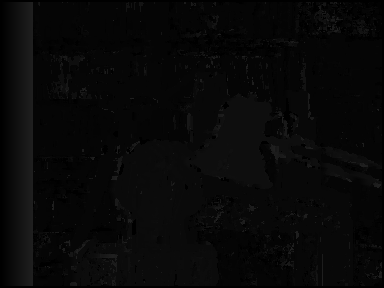
\includegraphics[width=5cm]{leftDisparity.png}
 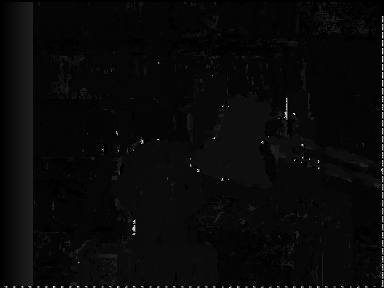
\includegraphics[width=5cm]{rightDisparity.png}
 \caption{Disparité de l'image gauche et de l'image droite}
\end{figure}
On peut voir apparaître, sur ces deux images, la forme de la statue et de la lampe qui sont
tous les deux les objets qui semblent être les plus proches des objectifs dans les images.

\section{Vérification gauche-droite}
Maintenant que nous avons calculé les disparités des deux images, nous effectuons une vérification
de cohérence gauche-droite. Pour cela, il suffit de vérifier que la valeur d'un pixel à une position (x,y)
dans l'image gauche est égale à la valeur du même pixel (x+shift,y) dans l'image droite. La valeur
shift étant la disparité du pixel de l'image droite en (x,y). Si les pixels de l'image gauche et de 
l'image droite ont la même valeur on met un 0 dans le masque à la position du pixel dans l'image gauche,
sinon on met la valeur 255. Voici le code correspondant à cette méthode :
\begin{lstlisting}[caption=Vérification de cohérence gauche-droite]
Mat iviLeftRightConsistency(const Mat& mLeftDisparity,
                             const Mat& mRightDisparity,
                             Mat& mValidityMask) {
     Mat mDisparity(mLeftDisparity.size(), CV_8U);
 
     int sizeX = mRightDisparity.cols;
     int sizeY = mRightDisparity.rows;
 
     for(int x = 0;  x < sizeX; x++) {
         for(int y = 0; y < sizeY; y++) {
             double left = (double)mLeftDisparity.at<unsigned char>(y,x);
             double shift = (double)mRightDisparity.at<unsigned char>(y,x);
             double right = (double)mRightDisparity.at<unsigned char>(y,x+shift);
             if(left >= right-1 && left <= right+1) {
                 mValidityMask.at<unsigned char>(y,x) = 0;
                 mDisparity.at<unsigned char>(y,x) = left;
             } else {
                 mValidityMask.at<unsigned char>(y,x) = 255;
                 mDisparity.at<unsigned char>(y,x) = 255;
             }
         }
     }
     return mDisparity;
 }
\end{lstlisting}

\begin{figure}[!h]
 \centering
 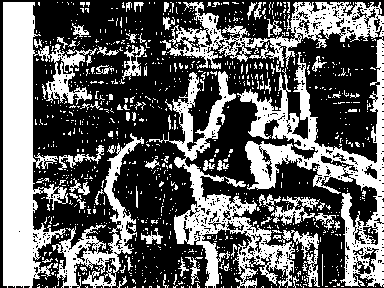
\includegraphics[width=7cm]{validityMask.png}
 \caption{Résultat de la vérification de cohérence gauche-droite}
\end{figure}

On voit que le résultat comporte beaucoup de pixel noire, ce qui signifie que la vérification est correcte.
Les pixels blancs qui nous permettent de distinguer les formes de la statue et de la lampe sont des faux appariements
du aux pixels occultés.

\section{Conclusion}
La méthode que nous avons analysée lors de ce TP est très efficace pour déterminer les pixels occultés, mais elle nécessite
d'avoir de l'équipement bien réglé afin d'obtenir des matrices intrinsèques équivalentes pour les deux objectifs.
\newpage
\section{Annexes}
\subsection{Annexe A}
\label{imageDroite}
\begin{lstlisting}[caption=Calcul de la SSD pour l'image droite]
Mat iviComputeRightSSDCost(const Mat& mLeftGray,
                            const Mat& mRightGray,
                            int iShift,
                            int iWindowHalfSize) {
     Mat mRightSSDCost(mLeftGray.size(), CV_64F);

     int sizeX = mRightGray.cols - iWindowHalfSize;
     int sizeY = mRightGray.rows - iWindowHalfSize;
 
     for(int x = iWindowHalfSize;  x < sizeX; x++) {
         for(int y = iWindowHalfSize; y < sizeY; y++) {
 
             double ssd = 0.0;
 
             for(int i = -iWindowHalfSize; i < iWindowHalfSize; i++) {
                 for(int j = -iWindowHalfSize; j < iWindowHalfSize; j++) {
 
                     if(x - iShift >= iWindowHalfSize) {
 
                         double il = (double)mLeftGray.at<unsigned char>(y+i, x+j-iShift);
                         double ir = (double)mRightGray.at<unsigned char>(y+i, x+j);
 
                         ssd += pow(ir - il, 2.0);
 
                     }
                 }
             }
 
             mRightSSDCost.at<double>(y,x) = ssd;
         }
     }
     return mRightSSDCost;
 }
\end{lstlisting}
\end{document}
